% % -----------------------------------------------------------------------------
\section{Overview of SBOL}
% % -----------------------------------------------------------------------------
Typically, information about a  genetic circuit includes the order of its constituents and their descriptions. The exact locations of these constituents and their sequences allow genetic circuits to be defined unambiguously, and reused in other designs. Interactions between these constituents are then used to construct biologically plausible designs. 
\Ctodo{reword for better clarity and coverage of the model -JSB}

% In the figure below, a simple toggle switch system is displayed, in which LacI and TetR repress each other's genes transcriptionally. The toggling of the system  is controlled by adding IPTG to deactivate LacI, and ATC to deactivate TetR. The components of the system includes genetic elements, proteins, small molecules.

\begin{figure}[ht]
\begin{center}
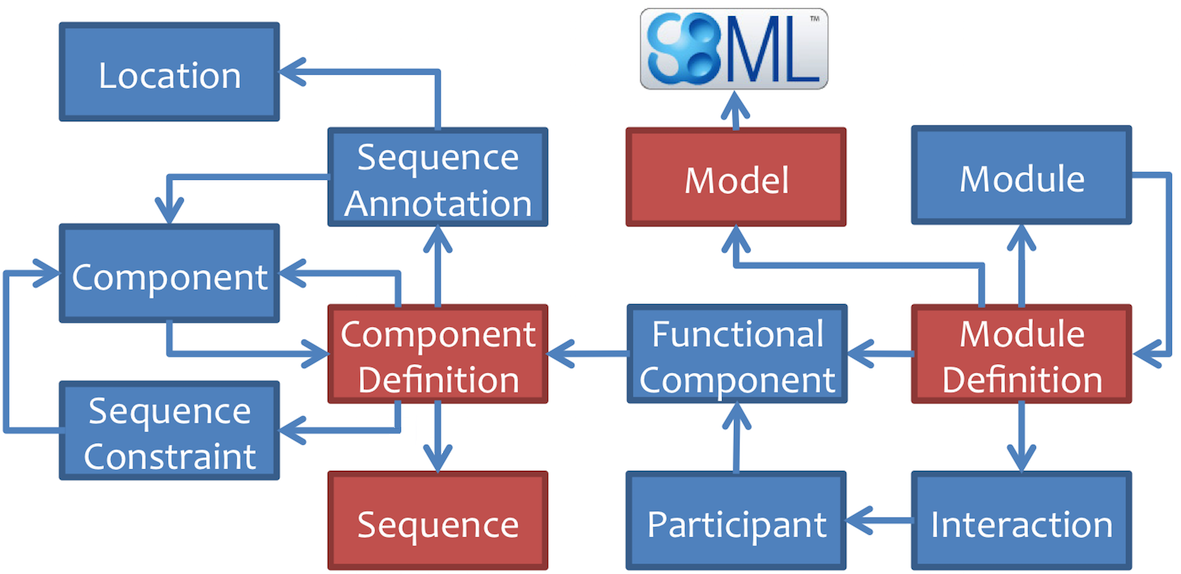
\includegraphics[scale=1.2]{images/SBOL2_2_revised.png}
\caption[]{ }
\label{images:overview}
\end{center}
\end{figure}
\Ctodo{Put a caption on the figure -JSB}
\LDtodo{Remove SBML from the figure -JSB}

The \sbol{Sequence} is a fundamental information object for synthetic biology and is needed to reuse components, to replicate synthetic biology work, and to assemble new synthetic biological systems. 
Therefore, both experimental work and theoretical sequence composition research depend heavily on the sequence associated with component definitions.

\Ctodo{need to make it clear that it includes DNA, RNA, and protein, also smooth the text --JSB}

SBOL includes different entities to describe such genetic circuits. Genetic elements such as promoters, RBS, CDSs and terminators are defined with the \sbol{ComponentDefinition} entity. Their instances are reused in different designs via the \sbol{Component}s that refer to corresponding \sbol{ComponentDefinition}s. \sbol{ComponentDefinition}s can also represent proteins, RNAs or small molecules. They are associated with sequence information such as nucleotides aminoacids or chemical structure. A full description of a genetic circuit is then represented using  \sbol{ModuleDefinition}s which contains information about molecular interactions and their participating components. Modules can be associated with quantitative or qualitative models using the \sbol{Model} entity, which is used to point to the actual location of a model.

\Ctodo{Need to also explain annotation --JSB}

SBOL facilitates the design of complex systems using hierarchical composition. In addition to using simple genetic elements in a modular fashion, modules that are composed of multiple, different components can also be reused. Such modules can expose some of the design components as inputs and outputs, which can be connected to components from other modules using \sbol{MapsTo} entities.

\Ctodo{This needs to be clarified.  Do we really want to explain MapsTo here? -JSB}

\Ctodo{Explain why it is important to separate definitions from instantiations?}

\LDtodo{The motivation for separating structural and functional considerations is not explained.  Which class names are structural, which class names are functional, and how are the two connected?  Do all structural components require a functional counterpart?  If not, explain why only a subset of structural components would have functional definitions.}

\Ctodo{As a person reading about SBOL2 for the first time, I rank this as the most important section.  This is your chance to concisely tell someone who won't read the whole document about the take-home messages for the new data model.}

\LDtodo{Why are URI's needed for Components?  Why not just for ComponentDefinitions?  Is there anything in SBOL that does not require a URI?}

\Dtodo{where did the XML-RDF section go?}

% The same toggle switch is now displayed using two LacI and TetR inverter submodules in figure \ref{images:toggleswitch_modular}. The LacI inverter uses LacI as input and produces the TetR output, and the TetR inverter uses TetR as input and produces the LacI output. These inputs and outputs are mapped in a parent module.

% Removed as redundant:
%-----------------------------------------------------------------------------
%\section{Introduction}
% -----------------------------------------------------------------------------
%While the first version of the Synthetic Biology Open Language (SBOL) has been adopted by several academic and commercial genetic design automation (GDA) software tools, it only covers a limited range of the requirements for a standardized exchange format for synthetic biology. The SBOL 2.0 specification revises version 1.1, enabling the representation of a wider range of components with and without sequences, including RNA components, protein components, small molecules, and molecular complexes. Additionally, the latest SBOL can be used to convey the intended function of a design, as well as its structural composition. 
%This dichotomous representation of the structural and functional features of a design is a paradigm applied to great success in electrical and computer engineering, and is essential for the development of design automation software in synthetic biology.
%
%The goal of this specification is to define the terminology and relationships used to describe biological designs. In order to provide a shared understanding between engineers seeking to exchange biological designs, SBOL provides a common definition of the concepts needed. As much as possible, we attempt to make explicit the meaning of all terminology and data structures.


% % -----------------------------------------------------------------------------
% \section{Overview of SBOL}
% % -----------------------------------------------------------------------------
% Typically, information about a  genetic circuit includes the order of its constituents and their descriptions. The exact locations of these constituents and their sequences allow genetic circuits to be defined unambiguously, and reused in other designs. Interactions between these constituents are then used to construct biologically plausible designs. 

% In the figure below, a simple toggle switch system is displayed, in which LacI and TetR repress each other's genes transcriptionally. The toggling of the system  is controlled by adding IPTG to deactivate LacI, and ATC to deactivate TetR. The components of the system includes genetic elements, proteins, small molecules.

% \begin{figure}[ht]
% \begin{center}
% 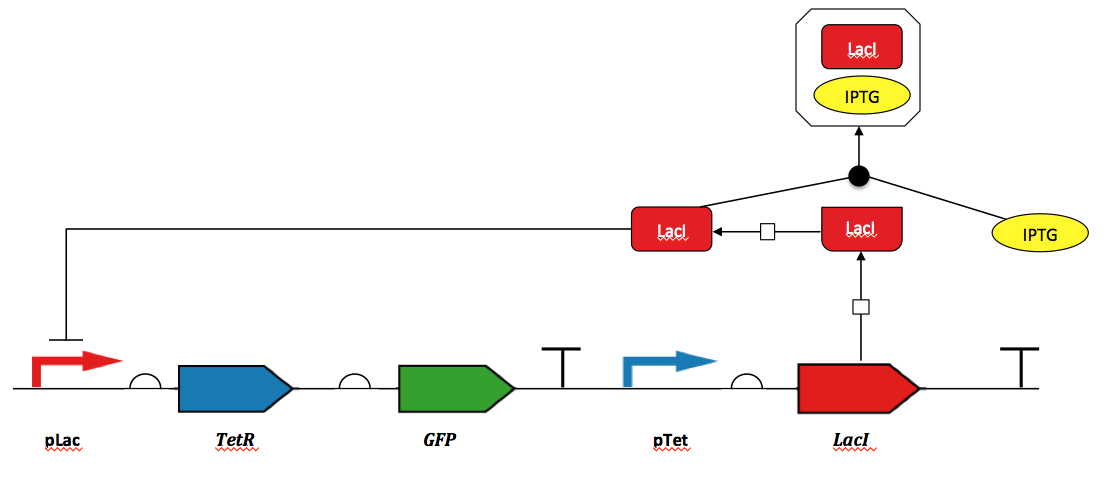
\includegraphics[scale=0.4]{images/toggleswitch_flat}
% \caption[]{An example toggle swicth genetic circuit. }
% \label{images:toggleswitch_flat}
% \end{center}
% \end{figure}

% SBOL includes different entities to describe such genetic circuits. Genetic elements such as promoters, RBS, CDSs and terminators are defined with the \sbol{ComponentDefinition} entity. Their instances are reused in different designs via the \sbol{Component}s that refer to corresponding \sbol{ComponentDefinition}s. \sbol{ComponentDefinition}s can also represent proteins, RNAs or small molecules. They are associated with sequence information such as nucleotides aminoacids or chemical structure. A full description of a genetic circuit is then represented using  \sbol{ModuleDefinition}s which contains information about molecular interactions and their participating components. Modules can be associated with quantitative or qualitative models using the \sbol{Model} entity, which is used to point to the actual location of a model.


% SBOL facilitates the design of complex systems using hierarchical composition. In addition to using simple genetic elements in a modular fashion, modules that are composed of multiple, different components can also be reused. Such modules can expose some of the design components as inputs and outputs, which can be connected to components from other modules using \sbol{MapsTo} entities.

